\section{Introduction}

The first work, which is today assigned to the field of artificial intelligence (AI), was done in 1943 by McCulloch and Pitts \cite{McCulloch1943}.
In their work they were inspired by neurons in the brain and created first mathematical formulations which later had a great influence on the development of neural networks.
The neurons are seen as switches whose activation is influenced by other neurons.
In this way complex systems can be created, which are able to solve different tasks.
The term artificial intelligence itself was coined by McCarthy in 1956, when he organized a two-month workshop in Dartmouth \cite{McCarthy1955}.

After the initial high expectations of artificial intelligence, without delivering the promised results, the field received less attention.
A famous quote from Herbert Simon in 1957 states: 
\begin{quotation}
    It is not my aim to surprise or shock you – but the simplest way I can summarize is to say that there are now in the world machines that think, that learn and that create. Moreover, their ability to do these things is going to increase rapidly until – in a visible future – the range of problems they can handle will be coextensive with the range to which the human mind has been applied.
\end{quotation}

However, contrary to these exaggerations, progress has been made over the decades.
After another period of high investment in the 1980s, without achieving the ambitious goals, the so-called "AI winter" set in, which was characterized by a lack of academic and economic interest and lack of funding.

Recently, however, research and application of these techniques have been attracting more attention.
This is due to a number of factors that are prevalent today.
One is the sheer amount of computing power that modern computers can have.
Even home computers today are capable of training models of remarkable complexity.

Furthermore, the amount of data available through the Internet facilitates the training of AIs for various tasks.
In order to train a model for a specific task, appropriate data are needed to make correct predictions about data never seen before (generalization).
Since data is available in large quantities, there are accordingly several databases for research, training and evaluation.
A list of databases can be found at \aka{https://en.wikipedia.org/wiki/List_of_datasets_for_machine-learning_research}.

That is why more and more attention is being paid to artificial intelligence in research, and more and more practical areas regard this technology as a solution to a wide range of problems.
Whether the recent enthusiasm is just exaggerated expectations, or whether the "last invention of mankind" \cite{Good1965} remains to be seen.

The term artificial intelligence is used to describe machine processes that perform tasks that are otherwise characteristic of human intelligence.
This paper is mainly intended to deal with a subfield of artificial intelligence, the so-called "deep learning".
This connection is shown in figure \ref{fig:ai_ml_dl}.

\begin{figure}
    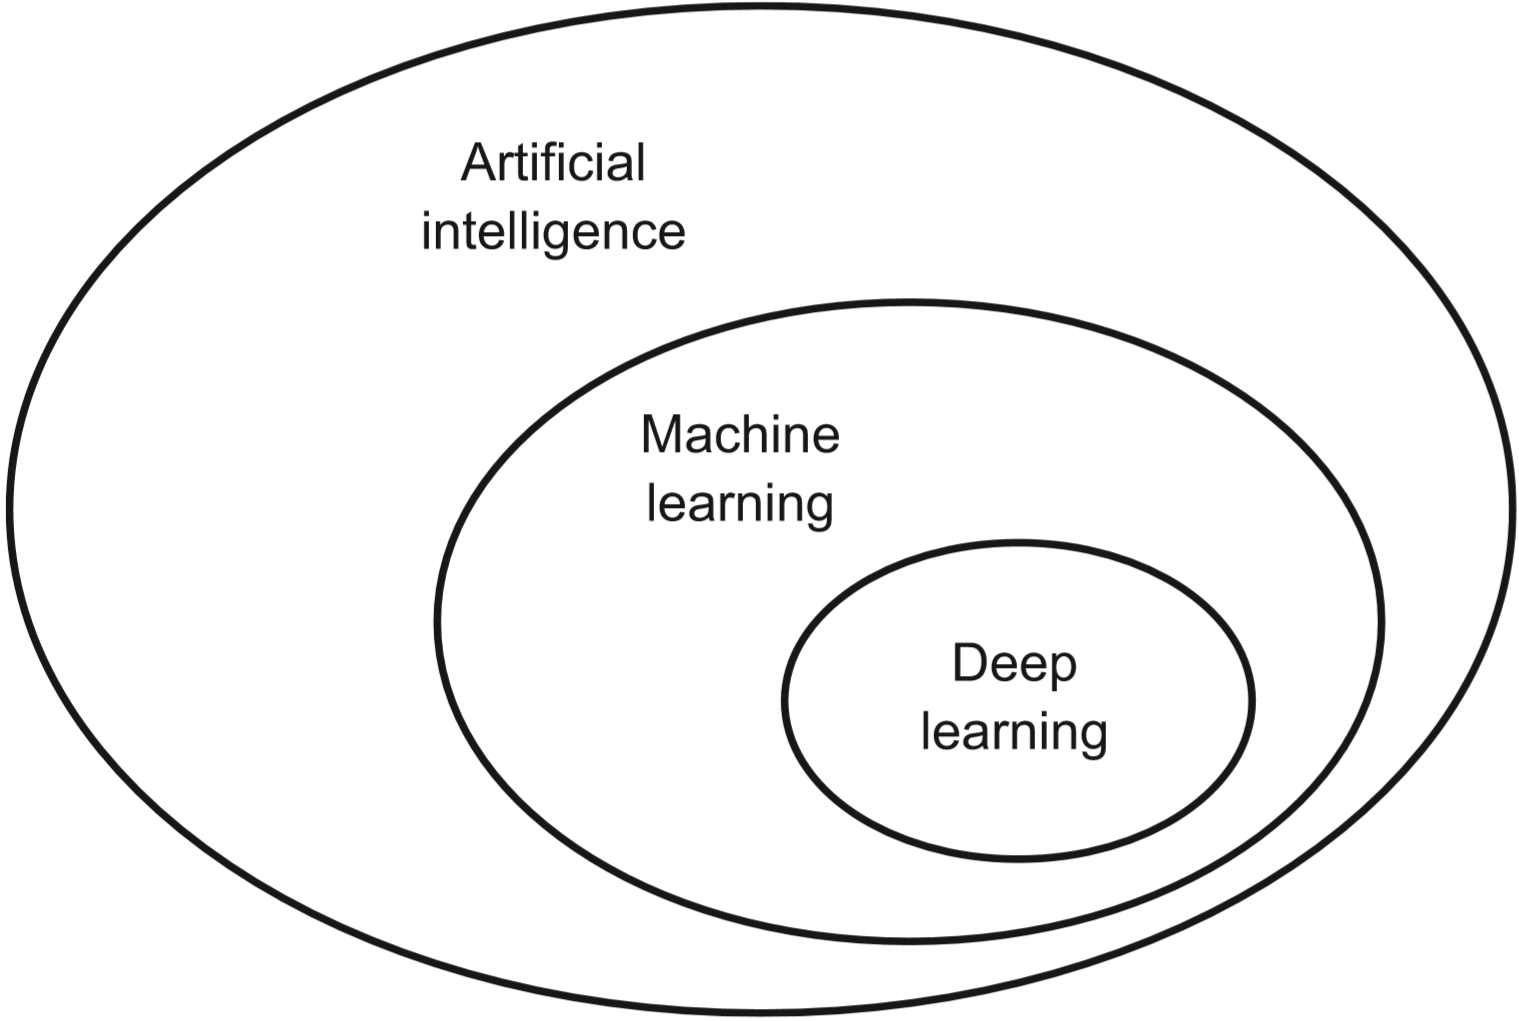
\includegraphics[width=0.5\textwidth]{images/ai_ml_dl.png}
    \caption[AI, ML and DL]{Artificial intelligence, machine learning and deep learning \cite[p.4]{Chollet2017}}
    \label{fig:ai_ml_dl}
\end{figure}

In this project I want to introduce machine learning into the field of kinematics for two-dimensional sketching and prototype development with \name{deepmech}.
The first solution implemented for this project takes images as input and outputs the respective type of handwritten mechanical symbols.
The models created with the presented approach are small and mostly independent of the used programming language, which is made possible by using the popular Keras \cite{Chollet} library on TensorFlow \cite{Google2019}.

Simple demonstrations are performed using JavaScript to connect to an emerging area of kinematics using web technologies such as \name{mec2} \cite{Goessner2019} and \name{mecEdit} \cite{Uhlig2019}.
For the training of the current model the Python implementation of TensorFlow is used, because the better utilization of the GPU with CUDA \cite{nvidia2019} as backend allows a faster training of the Keras models.
Thanks to the convertibility of model descriptions for use in different programming languages, this allows seamless transitions between different approaches.

Before showing how deepmech was developed, the basics of machine learning will be covered, with some simple examples as an introduction, introducing the general terminology used in this paper.
In chapter 3 the concepts are expanded by introducing neural networks, which are the key to translating the workings of machine learning into practical models.
Another topic to be covered is data generation.
Data is an important part of the training of statistical models, so data generation and augmentation is covered in chapter 4.
Then the first working model is shown.
All main components of the process are examined in detail to get a better understanding of each function.
Chapter 6 deals with optimizing the model to improve accuracy and minimize the size of the model that will be loaded in future applications.
Finally, a conclusion is given in which the results are evaluated.
